\section{Connected spaces, Hausdorff spaces, compact spaces.}
14.02

\subsection{Hausdorff spaces}

\begin{definition}[Hausdorff]
    A space \( X \) is Hausdorff if
    \( \forall x, y \in X , x \neq y\)
    there exists open subsets \( U, V \subseteq X \)
    with \( x \in U \) and \( y \in V \) and \( U \cap V = \emptyset \).
\end{definition}

\begin{example}
    Every discrete space is Hausdorff.
\end{example}

\begin{nonexample}
  \( X = \{ a, b, c \}, \tau = \{ \emptyset, X, \{a\}, \{a, b\}  \} \) is not Hausdorff.
\end{nonexample}

\begin{nonexample}
  \( X \) with the indiscrete topology, \( \abs{X} > 1 \), is not Hausdorff.
\end{nonexample}

\begin{proposition}
   Every metric space is Hausdorff. 
\end{proposition}

\begin{proof}
    Let \( X \) be a metric space.
    Let \( x, y \in X, x \neq y \).
    Let \( \varepsilon = d(x, y) \). Then \( d(x, y) > 0 \).
    Construct balls around \( x, y \) with radius \( \delta = \epsilon/2 \).
    Then you win.
\end{proof}

\begin{theorem}
    Let \( X \) be a Hausdorff space.
    Then the subset \( \{ x \} \subseteq X  \)
    is closed for all \( x \in X \).
\end{theorem}

\begin{proof}
  Pick \( x \in X \).
  Let \( y \in \{ x \} ^\mathsf{c} \).
  Since \( X \) Hausdorff,
  there exists open subsets \( U, V \subseteq X \)
  such that \( x \in U, y \in V, U \cap V = \emptyset \).
  Since \( x \notin V \), \( V \subseteq \{ x \} ^\mathsf{c} \).
  Since \( y \) was arbitrary, \( \{ x \} ^\mathsf{c} \)
  is open, so \( \{ x \}  \) is closed. Since \( x \) was
  arbitrary this holds for all \( x \in X \).
\end{proof}

\begin{theorem}
    Let \( X, Y \) be a Hausdorff space.
    Then \( X \times Y \) is Hausdorff.
\end{theorem}

\begin{proof}
  Pick \( (x_1, y_1), (x_2, y_2) \subseteq X \times Y \).
  Since \( X \) is Hausdorff, so
  there exists opens \( U \ni x_1, V \ni x_2 \), \( U \cap V = \emptyset \).
  Now we have opens \( U \times Y \ni (x_1, y_1) \), 
  \( V \times Y \ni (x_2, y_2) \) such that
  \[
    (U \times Y) \cap (V \times Y)
    = (U \cap V) \times Y
    = \emptyset \times Y
    = \emptyset
  \]
\end{proof}

\begin{theorem}
   Let \( X \) be Hausdorff.
   Let \( A \subseteq X \) be a subspace.
   Then \( A \) is Hausdorff.
\end{theorem}

\begin{proof}
  Let \( x, y \in A \).
  Since \( X \) Hausdorff, there exists
  opens \( U \ni x, V \ni y \),
  \( U \subseteq X, V \subseteq X \).
  Now \( U \cap A \ni x \) and \( V \cap A \ni y \)
  are opens in \( A \) and
  \[
    (U \cap A) \cap (V \cap A) = (U \cap V) \cap A = \emptyset
  \]
\end{proof}

\begin{theorem}
    Let \( X \) be a topological space.
    \( X \) is Hausdorff iff. \( \Delta \subseteq X \times X, \Delta = \{ (x, x) \mid x\in X \} \)
    is closed.
\end{theorem}

\begin{proof}
   We show both directions.
   \begin{enumerate}
     \item[\( \Rightarrow \))]
       Assume \( X \) is Hausdorff.
       Claim: \( \Delta^\mathsf{c} \) is open.
      Pick \( (x, y) \in \Delta^\mathsf{c} \).
      Since \( x \neq y \) and \( X \) Hausdorff
      we can find opens \( U \ni x, V \ni y \) such that
      \( U \cap V = \emptyset \). Now, \( (x, y) \in U \times V \),
      but we need to show that \( U \times V \subseteq \Delta ^\mathsf{c} \).
      Suppose \( (a, b) \in U \times V \) and \( (a, b) \in \Delta \).
      Then \( a = b \), but \( U \cap V = \emptyset \), which is a contradiction.
      Hence \( U \times V \subseteq \Delta^\mathsf{c} \).
      \( (x, y) \) was arbitrary, so \( \Delta^\mathsf{c} \) is open,
      hence \( \Delta \) is closed.
     \item[\( \Leftarrow \))]
       Assume \( \Delta \) is closed.
       Then \( \Delta^\mathsf{c} \) is open.
       That is, for every \( x \neq y \),
       \( (x, y) \in \Delta^\mathsf{c} \),
       and we can find a open \( U \times V \ni (x, y) \).
       Suppose \( U \cap V \neq \emptyset \).
       Then there exists a point \( z \in U, z \in V \).
       But then \( (z, z) \in U \times V \) and \( (z, z) \in \Delta \),
       which is a contradiction. So \( U \cap V = \emptyset \).
       Hence, \( X \) is Hausdorff.
   \end{enumerate}
\end{proof}

\begin{definition}[cover]
   Let \( X \) be a topological space. 
   We say that a \( I \)-indexed familiy
   of opens in \( X \), \( \{ U_i  \}_{i \in I} \),
   is a cover of \( X \) if
   \[
     \bigcup_{i\in I} U_i = X
   \]
\end{definition}

\begin{definition}[refinement]
   Let \( X \) be a topological space
   and let \( \{ U_i  \}_{i\in I}  \)
   be a cover.
   Let \( J \subseteq I \).
   We say that the \( J \)-indexed
   family \( \{ U_j \}_{j \in J} \)
   is a refinement of \( \{ U_i \}_{i \in I} \)
   if
   \[
     \bigcup_{j \in J} U_j = X
   \]
\end{definition}

\begin{definition}[compact space]
   A space \( X \) is compact if
   every cover \( \{ U_i \}_{i \in I}  \)
   admits a refinement \( J \subseteq I \)
   with \( \abs{J} < \infty \).
\end{definition}

\begin{nonexample}
   \( \mathbb{R} \) is not compact. 
\end{nonexample}

\begin{proof}
  \( \{ (-n, n) \}_{n \in \mathbb{N}}  \) is a cover.
  Sps. \( \mathbb{R} \) is compact.
  Then there exists a finite subset of \( \mathbb{N} \), say \( J \),
  that covers \( \mathbb{R} \).
  Let \( r \) be the maximum of \( J \).
  Then \( \abs{x} < r \) for all \( x \in \mathbb{R} \),
  which is absurd.
  So \( \mathbb{R} \) is not compact.
\end{proof}

\begin{example}
    \( X \) finite topological space. Then \( X \) is compact.
\end{example}

\begin{example}
   \( X \) indiscrete topology. Then \( X \) compact. 
\end{example}

\begin{definition}[compact subspace]
    Let \( A \subseteq X \) be a subspace.
    Then \( A \) is compact in \( X \) 
    if it is compact in the subspace topology.
\end{definition}

\begin{lemma}
  \label{lma:subspace_compact}
    Let \( A \subseteq X  \) be a subspace.
    Then \( A \) is compact as a subspace iff.
    given a family \( \{ U_i \}_{i \in I} \), \( U_i \)
    open in \( X \) and \( A \subseteq \bigcup_{i \in I} U_i \), then
    there exists a finite refinement \( J \subseteq I \) such that
    \[
      A \subseteq \bigcup_{j \in J} U_j
    \]
\end{lemma}

\begin{center}
  \label{pic:fin_cover}
  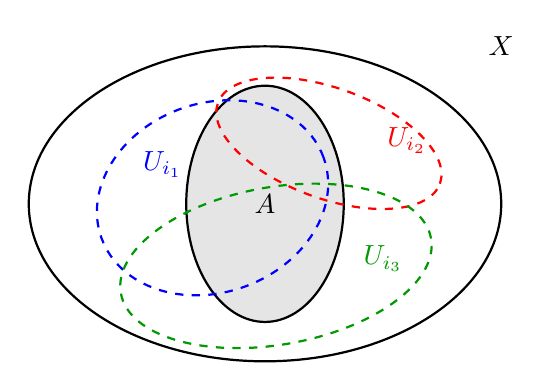
\begin{tikzpicture}
    % Draw the large space X
    \draw[thick] (0,0) ellipse (3 and 2);
    \node at (3, 2) {$X$};

    % Draw the compact subspace A
    \draw[thick, fill=gray!20] (0,0) ellipse (1 and 1.5);
    \node at (0, 0) {$A$};

    % Draw open sets U_i that cover A
    \draw[blue, thick, dashed, rotate=20] (-0.6,0.3) ellipse (1.5 and 1.2);
    \node[blue] at (-1.3,0.5) {$U_{i_1}$};

    \draw[red, thick, dashed, rotate=-20] (0.5,1) ellipse (1.5 and 0.7);
    \node[red] at (1.8, 0.8) {$U_{i_2}$};

    \draw[green!60!black, thick, dashed, rotate=10] (0,-0.8) ellipse (2 and 1);
    \node[green!60!black] at (1.5,-0.7) {$U_{i_3}$};
  \end{tikzpicture}
\end{center}

\begin{proof}
    We show both directions.
    \begin{enumerate}
      \item[\( \Rightarrow \))]
        Assume \( A \) is compact as
        a subspace.
        Let \( \{ U_i \} _{i \in I}\) be a familiy
        of opens in \( X \) such that
        \( A \subseteq \bigcup_{i \in I} U_i \).
        Then \( \bigcup_{i \in I} U_i \cap A \)
        covers \( A \) since
        \[
          \bigcup_{i \in I} U_i \cap A = A \cap \bigcup_{i \in I} U_i = A
        \]
        Now, since \( A \) is compact as a subspace,
        there exists a finite refinement \( J \subseteq I \)
        such that
        \[
          A = \bigcup_{j \in J} U_j \cap A
          \subseteq \bigcup_{j \in J} U_j
        \]
      \item[\( \Leftarrow \))]
        Assume that every family \( \{ U_i \} _{i \in I} \)
        such that \( A \subseteq \bigcup_{i \in I} U_i \)
        admits a finite refinement \( J \subseteq I \) such that
        \[
          A \subseteq \bigcup_{j \in J} U_j
        \]
        Then we need to show that \( A \) is compact as 
        a subspace.
        Pick a cover of \( A \):
        \[
          \{ V_i \}_{i \in I} = \{ U_i \cap A \}_{i \in I}
        \]
        Since \( A \subseteq \bigcup_{i \in I} U_i \),
        then by  assumtion we can refine it and get
        \[
          A = \bigcup_{\alpha = 0}^n V_{i_\alpha}
        \]
    \end{enumerate}
\end{proof}

\begin{theorem}
  \label{thm:compace_sub_closed}
    Let \( X \) be a compact space.
    Let \( A \subseteq X \) be closed.
    Then \( A \) is compact.
\end{theorem}

\begin{proof}
  Let \( \{ U_i \}_{i \in I}  \) be a family of opens such that
   \( A \subseteq \bigcup_{i \in I} U_i \).
    Now since \( A \) closed, then \( A^\mathsf{c} \)
    open. We have that
    \[
      \bigcup_{i \in I} U_i \cup A^\mathsf{c} = X
    \]
    and since \( X \) compact, we have a finite refinement
    \( J \subseteq I \cup *  \).
    Now, \( J \) contains finitely many indices such that
    \( A \subseteq \bigcup_{j \in J} U_j \)
    and by lemma \ref{lma:subspace_compact}, \( A \) is compact.
\end{proof}

\begin{theorem}
  \label{thm:compact->closed}
    Let \( X \) be Hausdorff.
    Given \( K \subseteq X \), \( K \) compact.
    Then \( K \) is closed.
\end{theorem}

\begin{proof}
    Since \( X \) is Hausdorff, we can do the following.
    Let \( x \notin K \).
    For every \(y \in K \),
    pick nbhs. \( U_y \ni x, V_y \ni y \)
    such that \( U_y \cap V_y = \emptyset \).
    Now \( \{ V_y \}_{y \in Y} \) is a cover of \( K \).
    Since
    \( K \) is compact, there exists a finite refinement
    \( J \) such that
    \[
      K \subseteq \bigcup_{j \in J} V_{y_j}
    \]
    Now, let \( U = \cap_{j\in J} U_{y_j} \).
    Note that \( x \in U \) and \( U \) is open.
    Also
    \[
      U \cap K \subseteq U \cap \left(\bigcup_{j \in J} V_{y_j}\right) = \bigcup_{j \in J} U \cap V_{y_j} = \emptyset
    \]
    Since \( x \notin K \) was arbitrary
    \( K^\mathsf{c} \) is open, hence \( K \) is closed.
\end{proof}

Motivation: this theorem makes life easier when we want to prove that
a surjective map is a quotient map by 
combining \ref{thm:compact->closed} and \ref{thm:cont_surj_closed->quotient}.
Here is an example:

\begin{example}
  We want to show that
  \begin{align*}
    f: [0, 1] &\longrightarrow \mathbb{S}^1 \\ t &\longmapsto (\cos 2 \pi t, \sin 2 \pi t)
  \end{align*}
  is a quotient map. 
\end{example}

\begin{proof}
  \( f \) is continuous and surjective.
  Let \( K \subseteq [0, 1] \) closed.
  Since \( [0, 1] \) compact and \( K \) is closed,
 \( K \) is compact by theorem \ref{thm:compace_sub_closed}.
  Now, \( f(K) \subseteq \mathbb{S}^1 \) and since
  \( \mathbb{S}^1 \) is Hausdorff we get that
  \( f(K) \) is closed by theorem \ref{thm:compact->closed}.
  Hence \( f \) is a continuous, surjective and closed map,
  so \( f \) is a quotient map by \ref{thm:cont_surj_closed->quotient}.
\end{proof}

